\documentclass[11pt,a4paper]{article}
\usepackage{enumitem}
\usepackage{graphicx}           % Extended \includegraphics         
\usepackage[reqno]{amsmath}            % Higher mathematics
\usepackage{hyperref}           
\usepackage[margin = 0.5in]{geometry}
\usepackage{float}
\usepackage{amssymb}            % special math fonts
\usepackage{amsmath}
\usepackage{siunitx}
\usepackage{enumitem}
\usepackage{cancel}
\usepackage{braket}
\usepackage{tikz}
\usepackage{pgfplots}
\usepackage[final]{pdfpages}
\usepackage{physics}
\usepackage{subcaption}
\usepackage{bbm}
\usepackage{rotating}
\usepackage{listings}
\usepackage{color}

\definecolor{codegreen}{rgb}{0,0.6,0}
\definecolor{codered}{rgb}{0.6,0,0}
\definecolor{codeblue}{rgb}{0,0,0.6}
\definecolor{codegray}{rgb}{0.5,0.5,0.5}
\definecolor{codepurple}{rgb}{0.58,0,0.82}
\definecolor{backcolour}{rgb}{0.95,0.95,0.92}
 
\lstdefinestyle{mystyle}{
    backgroundcolor=\color{backcolour},   
    commentstyle=\color{codered},
    keywordstyle=\color{codeblue},
    numberstyle=\tiny\color{codegray},
    stringstyle=\color{codegreen},
    basicstyle=\footnotesize,
    breakatwhitespace=false,         
    breaklines=true,                 
    captionpos=b,                    
    keepspaces=true,                 
    numbers=left,                    
    numbersep=5pt,                  
    showspaces=false,                
    showstringspaces=false,
    showtabs=false,                  
    tabsize=2
}
 
\lstset{style=mystyle}

%\tikzexternalize[optimize=false,prefix=PREFIX]

\pgfplotsset{compat = 1.13}

\newcommand{\h}{\hat}
\newcommand{\hham}{\hat{\mathcal{H}}}

\begin{document}


\title{\bf PHYC90010 - Statistical Mechanics Assignment 2}
\author{Mitchell de Zylva - 756539}
\maketitle



\begin{center}
\vspace{1cm}
\rule{145mm}{0.5mm}
\vspace{1cm}
\end{center}
\tableofcontents
\newpage
%\input{/home/part3/mylatex/preamble}
\newpage

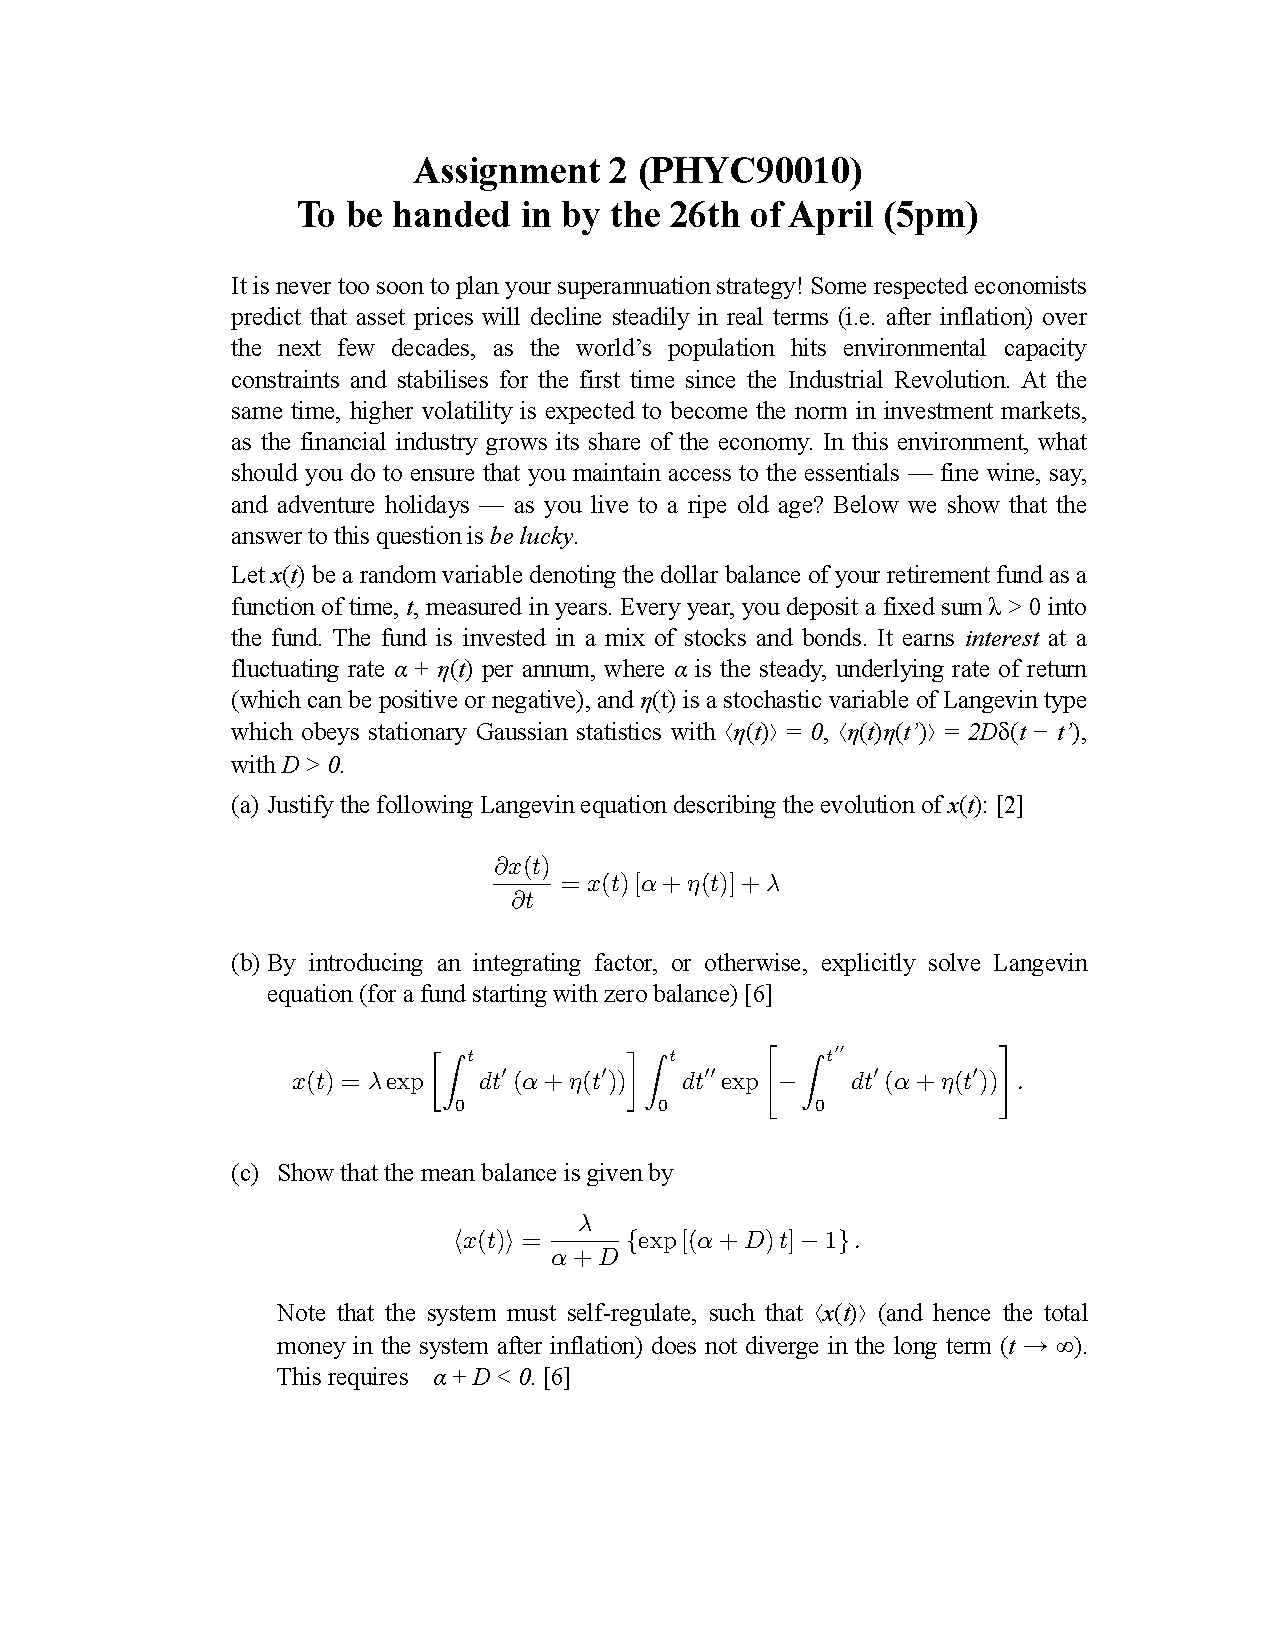
\includepdf[pages=-]{/home/mitchell/Documents/masters/statmech/second/Assign2_2019.pdf}


%%%%%%%%%%%%%%%%%%%%%%%%%%%%%%%%%%%%%%%%%%%%%%%%%%%%%%%%%%%%%%%%%%%%%%
\section{Question 1}
\label{sec:question1}
%%%%%%%%%%%%%%%%%%%%%%%%%%%%%%%%%%%%%%%%%%%%%%%%%%%%%%%%%%%%%%%%%%%%%%
%%%%%%%%%%%%%%%%%%%%%%%%%%%
\subsection{Question 1 - (a)}
\label{sec:question1:subsec:parta}
%%%%%%%%%%%%%%%%%%%%%%%%%%%
The rate of change of the amount in a super fund is by definition proportional to the previous amount in the super fund, i.e. 
$$\pdv{x(t)}{t} \propto x(t) .$$
The proportionality will be dependant on the static growth amount, which in this case is the interest, and some gaussian random noise component, making the strict equivalency 
$$\pdv{x(t)}{t} = x(t) [\alpha + \eta(t)] .$$
However, we also have to factor in the contributions made to the fund, which are some fixed element $\lambda$. This makes the final expression
\begin{align}\label{eq:langevin}
  \pdv{x(t)}{t} = x(t) [\alpha + \eta(t)] + \lambda
\end{align}
, as required.
%%%%%%%%%%%%%%%%%%%%%%%%%%%
\subsection{Question 1 - (b)}
\label{sec:question1:subsec:partb}
%%%%%%%%%%%%%%%%%%%%%%%%%%%
To solve this expression using an integrating factor, we need to rearrange the first order differential equation  so that it has the form 
$$ \pdv{x(t)}{t} + P x(t) = Q .$$
Doing so, we see that 
\begin{align*}
  P &= -[\alpha + \eta(t)] \\
  Q &= \lambda .
\end{align*}
Now if introduce an integrating factor, defined as 
\begin{equation}\label{eq:integ_factor}
  I = \exp{\int P dx},
\end{equation}
we can re-write our differential in the form 
$$I \pdv{x(t)}{t} + I P x = I Q, $$
and integrate both sides
$$\int \left[I \pdv{x(t)}{t} + I P x\right] dt = \int I Q dt . $$
Doing so allows us to take advantage of the product rule, whereby $\dv{t}(I x) = I \dv{x}{t} + I P x   $, which gives the solution to the differential as 
\begin{align*}
  I x & = \int I Q dt \\
  \rightarrow x(t) & = \frac{\int I Q dt}{I}
\end{align*}
Substituting $I = \exp{\int -[\alpha  + \eta(t)] dt}$ yields the expression 
\begin{align*}
  x(t) &= \frac{\int \lambda \exp[- \int_0^{t^\prime} \alpha + \eta(t^{\prime \prime}) dt^{\prime \prime} ]}{I} \\
  &= \lambda \exp[ \int_0^{t} \alpha + \eta(t^{\prime}) dt^{\prime} ]\int_0^t dt^{\prime \prime} \exp[- \int_0^{t^{\prime \prime}} \alpha + \eta(t^{\prime \prime}) dt^{\prime \prime} ] 
\end{align*}
, as required.

%%%%%%%%%%%%%%%%%%%%%%%%%%%
\subsection{Question 1 - (c)}
\label{sec:question1:subsec:partc}
%%%%%%%%%%%%%%%%%%%%%%%%%%%
We know that $\exp[\int_0^t \alpha + \eta(t^\prime) dt^\prime] $ doesn't depend on $dt^{\prime \prime}$, so we can move it inside the integral. Defining $\zeta (t) = \alpha + \eta(t)$, we see that the expression becomes

\begin{align*} 
x(t)  & =  \lambda \int_0^t dt^{\prime \prime}\exp[ \int_0^{t} \zeta(t^\prime) dt^{\prime} ] \exp[- \int_0^{t^{\prime \prime}} \zeta(t^{\prime \prime}) dt^{\prime \prime} ] \\
 = & \lambda \int_0^t dt^{\prime \prime}\exp[ \int_{t^{\prime \prime}}^{t} \zeta(t^\prime) dt^{\prime} ] .
\end{align*}
Now if we take the expecatation value of this expression, it becomes
\begin{align*}
 \left< x (t) \right> &=  \left<{\lambda \int_0^t dt^{\prime \prime}\exp[ \int_{t^{\prime \prime}}^{t} \zeta(t^\prime) dt^{\prime} ]} \right> . 
\end{align*}

We can pass the expectation value through the integral function, and all constants, since the expecation value of a number is just a number
\begin{align}\label{eq:exp_val}
&= \lambda \int_0^t dt^{\prime \prime}  \left<\exp[ \int_{t^{\prime \prime}}^{t} \zeta(t^\prime)  dt^{\prime} ]\right>
\end{align} 
In order to calculate this, we need to first characterise the argument of the exponent. Now, we know that $\zeta(t)$ is some shifted random gaussian variable. This essentially means that by taking the integral over some finite domain, we are in essence sampling the distribution, which is another gaussian 
%%% This doesn't make sense, need to find some way to quote this, because I don't know where it has come from %%%
% \par If we take out the $\alpha$ term, the above expression becomes
% \begin{align*}
%  &= \lambda \int_0^t dt^{\prime \prime} \exp{\alpha(t-t^{\prime \prime})}
%   \left<\exp[ \int_{t^{\prime \prime}}^{t} \eta(t^\prime)  dt^{\prime} ]\right>
% \end{align*}
This is basically the expecation value of the moment generating function. For some random gaussian variable, we know that this takes the form 
\begin{align*}
  \left< e^{pX} \right> &= \int_{-\infty}^\infty e^{px^\prime} \frac{1}{\sqrt{2 \pi \sigma^2}} \exp{\frac{-(x^\prime - \mu)^2}{2 \sigma^2}} d x^\prime.
\end{align*}
If we make a change of variable, letting $x = x^\prime - \mu$, and complete the square inside the exponential, this becomes
\begin{align*}
  &= \frac{\exp(p \mu)}{\sqrt{2 \pi \sigma^2}} \int_{-\infty}^{\infty} \exp(px) \exp(\frac{-x^2}{2 \sigma^2}) dx \\ 
  &= \frac{\exp(p \mu)}{\sqrt{2 \pi \sigma^2}} \int_{-\infty}^{\infty} \exp(\frac{-1}{2 \sigma^2} {x^2 - 2 \sigma^2 p x + \sigma^4 p^2 - \sigma^4 p^2}) dx \\
  &= \exp(p \mu + \frac{\sigma^2}{2} p) \frac{1}{\sqrt{2 \pi \sigma^2}} 
  \int_{\infty}^\infty \exp{\frac{- (x-\sigma^2 p^2)^2}{2 \sigma^2}} dx\\
  &= \exp(p \mu + \frac{\sigma^2}{2} p).
\end{align*}
Given that we know the form of the solution, we can see that in this case, 
\begin{align*}
  \mu &= \alpha ( t - t^{\prime \prime}), \\
  \sigma^2 &= 2D ( t - t^{\prime \prime}) \text{, and } \\
  p &= 1.
\end{align*}
This makes \eqref{eq:exp_val} into 
\begin{align*}
  &= \lambda \int_0^t dt^{\prime \prime} \exp((\alpha+D) (t - t^{\prime \prime}) ) \\
  &= \frac{\lambda}{\alpha + D} \left[ \exp((\alpha + D)(t - t^{\prime \prime}))\right]_0^{t^{\prime \prime} = t} \\
  &= \frac{\lambda}{\alpha + D} [\exp((\alpha+D)t) - 1]
\end{align*}
as required.

%%%%%%%%%%%%%%%%%%%%%%%%%%%
\subsection{Question 1 - (d)}
\label{sec:question1:subsec:partd}
%%%%%%%%%%%%%%%%%%%%%%%%%%%
In order to convert the Langevin Equation to the Fokker Planck Equation, we have to first make a change of variables. Considering $u = \log(x)$, we can make the substitution 
\begin{align*}
  \pdv{u}{t} &= \pdv{u}{x} \pdv{x}{t} \\
  &= \frac{1}{x} \pdv{x}{t} \\
  &= e^{-u} (e^u [\alpha + \eta(t)] + \lambda) \\
  &= [\alpha + \eta(t)] + \lambda e^{-u}
\end{align*} 
This has the general form of a standard Langevin equation. We know that for a given Langevin equation with the form 
\begin{equation}
  \label{eq:std_langevin}
  \pdv{x_i}{t} = A_i (x) + B_{ij}(x,t) \xi_j (t) 
\end{equation}
has a corresponding Fokker Planck Equation
\begin{equation}
  \label{eq:std_fkkrplnk}
  \pdv{p(x,t)}{x} = - \pdv{x_i} [A_i(x,t) p(x,t)] + \frac{1}{2}                 \frac{\partial^2}{\partial x_i \partial x_j} [B_{ik}(x,t) B_{jk} (x,t) p(x,t)].
\end{equation}
We can see that in this case, 
\begin{align*}
  A_i(u) &= \alpha + \lambda e^{-u} \text{ , and}\\
  B_{ij} (u) &= \lim_{\Delta t \rightarrow 0} \frac{1}{\Delta t} \left< \Delta \xi(t) \Delta \xi(t^\prime) \right> \\
  &= \lim_{\Delta t \rightarrow 0} \frac{1}{\Delta t} \int_0^{\Delta t} dt^\prime \int_0^{\Delta t^\prime} dt^{\prime \prime} \left< \xi(t^\prime) \xi(t^{\prime \prime}) \right> \\
  &= \lim_{\Delta t \rightarrow 0} \frac{1}{\Delta t} \int_0^{\Delta t} dt^\prime \int_0^{\Delta t^\prime} dt^{\prime \prime} 2 D \delta(t^\prime - t^{\prime \prime}) \\
  &= \lim_{\Delta t \rightarrow 0} 2 D \frac{1}{\Delta t} \int_0^{\Delta t} dt^\prime  \\
  &= \lim_{\Delta t \rightarrow 0} 2 D \frac{1}{\cancel{\Delta t}} \cancel{\Delta t}  \\
  &= 2D \\
\end{align*}
Making the corresponding Fokker Planck Equation into
\begin{equation}\label{eq:fkkr_plnck}
  \pdv{p(x,t)}{t} = - \pdv{u} [(\alpha + \lambda e^{-u}) p(u,t)] + D                 \frac{\partial^2}{\partial^2  u} [p(u,t)],
\end{equation}
as required.
%%%%%%%%%%%%%%\pdv{x_i}{t} = A_i (x) + B_{ij}(x,t) \xi_j (t) %%%%%%%%%%%%%
\subsection{Question 1 - (e)}
\label{sec:question1:subsec:parte}
%%%%%%%%%%%%%%%%%%%%%%%%%%%
If we consider that you cannot have a negative balance in a superannuation fund, the amount of money in the fund cannot go below zero, and so the system self-imposes a reflecting boundary at $x=0$

%%%%%%%%%%%%%%%%%%%%%%%%%%%
\subsection{Question 1 - (f)}
\label{sec:question1:subsec:partf}
%%%%%%%%%%%%%%%%%%%%%%%%%%%
For the steady state solution, we assume the $\pdv{p}{t} = 0$ and there is no $t$ dependence. This effectively reduces \eqref{eq:fkkr_plnck} to 
$$   0 = - \pdv{u} [(\alpha + \lambda e^{-u}) p(u)] + D                 \frac{\partial^2}{\partial^2  u} [p(u)].
$$ 
To solve this, we reduce this problem to a first order differential by integrating once
\begin{align*}
  \pdv{u} [(\lambda \exp(-u) + \alpha) q(u)] &= D \pdv[2]{q}{u} \\
  [\lambda \exp(- u) + \alpha] q(u) &= D \pdv{q}{u}.
\end{align*}
This is now a seperable first order differential equation, which we can now solve 
\begin{align*}
  \pdv{q}{u} &= \frac{e^{-u}( \alpha e^u + \lambda )q(u) }{D} \\
  \frac{D \pdv{q}{u}}{q(u)} &= e^{-u} ( \alpha e^u +\lambda) \\
  \int \frac{D \pdv{q}{u}}{q(u)} &= \alpha u - e^{-u} \lambda + c \\
  D \log(q(u)) &= \alpha u - e^{-u} \lambda + c \\
  \Rightarrow q_s(u) &= \exp((\alpha u - \lambda e^{-u} + c)/D)
\end{align*}
I am not entirely sure how to implement the reflecting boundary to constrain this class of solution. I know that it implies that 
$$ n \cdot \vec{J} = 0 $$
But it seems that this is just the same differential eqaution that I have already solved above. 
%%%%%%%%%%%%%%%%%%%%%%%%%%%
\subsection{Question 1 - (g)}
\label{sec:question1:subsec:partg}
%%%%%%%%%%%%%%%%%%%%%%%%%%%
%%%%%%%%%%%%%%%%%%%%%%%%%%%
\subsubsection{Question 1 - (g) - (i)}
\label{sec:question1:subsec:partg:subsub:i}
%%%%%%%%%%%%%%%%%%%%%%%%%%%
We know that the relationship between $u$ and $x$ is given by the expression $u = \ln(x)$, and so re-writing the steady state solution in terms of $x$ gives 
\begin{align*}
  q(x) &= \exp((\alpha \ln(x))- \lambda/x + c) \\
  &= \exp((\ln(x^\alpha))- \lambda/x + c) \\
  &= x^\alpha \exp(-\frac{\lambda}{x} + c)
\end{align*}

%%%%%%%%%%%%%%%%%%%%%%%%%%%
\subsubsection{Question 1 - (g) - (ii)}
\label{sec:question1:subsec:partg:subsub:ii}
%%%%%%%%%%%%%%%%%%%%%%%%%%%
\begin{figure}[H]\label{fig:steady_state}
  \centering
  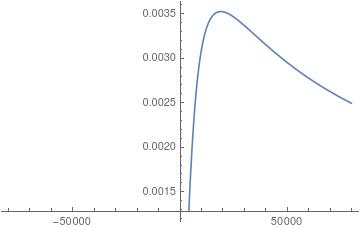
\includegraphics[scale=0.7]{/home/mitchell/Documents/masters/statmech/second/steady_state_big.jpeg}
  \caption{Steady State Solution for $\lambda = 10000$, $ \alpha + D = -0.52 $}
  \end{figure}
When we plot the steady state solution, we see that it grows steadily, before falling once a certain value is reached. These values are a result of the parameter choice, but the overall behaviour is preserved if different parameters are chosen. This climb and decay suggests that the steady state solution 

%%%%%%%%%%%%%%%%%%%%%%%%%%%
\subsubsection{Question 1 - (g) - (iii)}
\label{sec:question1:subsec:partg:subsub:iii}
%%%%%%%%%%%%%%%%%%%%%%%%%%%
If the system self regulates itself to be marginally stable, the variance doesn't diverge as you take $t \rightarrow \infty$. We still see some strange fluctuating behaviour towards later times. This suggests that even if the system regulates in the broadest sense, the fluctuations are very un-correlated at longer times.

\begin{figure}[H]
  \centering
  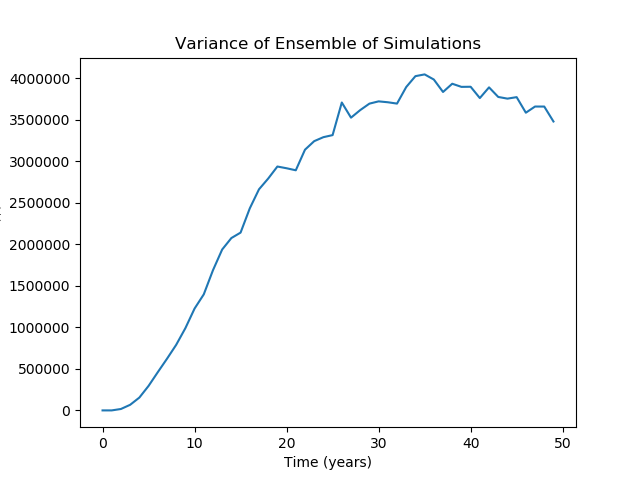
\includegraphics[scale=0.7]{/home/mitchell/Documents/masters/statmech/second/variance.png}
  \caption{Ensemble Mean of $1000$ simulations of $\lambda = 10000$, $ \alpha + D = -0.52 $, measured quarterly ($h = 0.25$) for 50 years}
  \label{fig:ensemble_variance}
\end{figure}

%%%%%%%%%%%%%%%%%%%%%%%%%%%
\subsubsection{Question 1 - (g) - (iv)}
\label{sec:question1:subsec:partg:subsub:iv}
%%%%%%%%%%%%%%%%%%%%%%%%%%%
In practice, this means that policy makers should always plan for the growth of superannuation funds to fall below the predicted growth of the economy. If they don't the funds are liable to diverge, which may lead to some sort of inflationary effects in the system. 

If this is not the case, then the mean of the funds diverges, which cannot occur practiaclly in an economy where you aren't printing money.
%%%%%%%%%%%%%%%%%%%%%%%%%%%
\subsection{Question 1 - (h)}
\label{sec:question1:subsec:parth}
%%%%%%%%%%%%%%%%%%%%%%%%%%%
I used the initial Langevin equation \eqref{eq:langevin}, and computed the behaviour of the superannuation using Euler Methods. In order to effectively find the behaviour of the super funds, we need to take the mean (and variance) of an ensemble of individual funds. What we notice is that the mean tends towards a certain value given sufficient time, with the $\lambda$ providing the yearly deposit, $\alpha$ providing the interest growth, and some chosen dispersion $D$. 

What I have noticed from the simulations, is that there is a consistent underestimation of the calculated values, when compared to the analytical values. It might be the case that this is simply a result of parameter selection, and I have not adequately selected values that are indicative of the ideal long term behaviour. 
\begin{figure}[H]
  \centering
  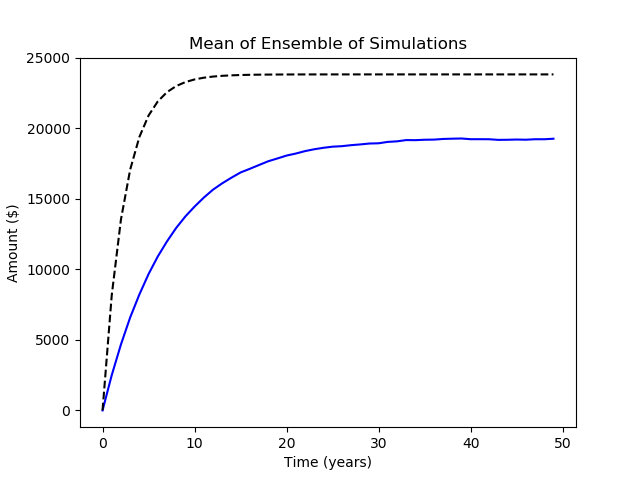
\includegraphics[scale=0.7]{/home/mitchell/Documents/masters/statmech/second/means.png}
  \caption{Ensemble Mean of $1000$ simulations of $\lambda = 10000$, $ \alpha + D = -0.52 $, measured quarterly ($h = 0.25$) for 50 years}
  \label{fig:ensemble_mean}
\end{figure}
\par When we compare the expected mean to the actual mean, we find that the expected mean overestimates the amount in the fund consistently. In Figure \ref{fig:ensemble_mean}, the dotted line is indicative of the expected value of the mean, and the solid line is the calculated mean. What we do see however, is that the long term behaviour appears to be the same, up to some scaling factor. This makes me think that it is a result of my parameter choice.

\medskip
\begin{figure}[H]
  \centering
  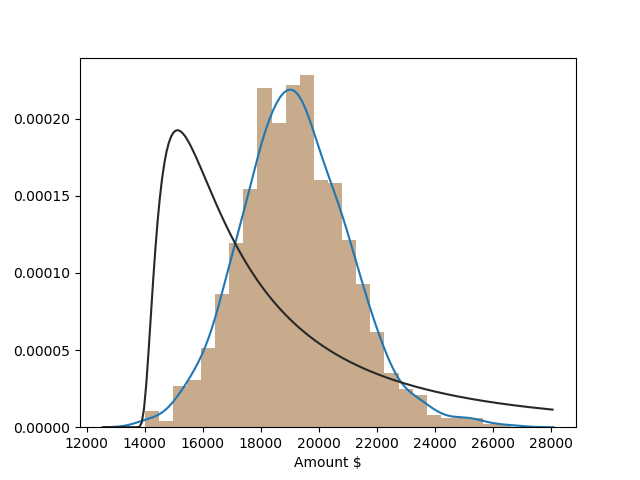
\includegraphics[scale=0.7]{/home/mitchell/Documents/masters/statmech/second/histogram.png}
  \caption{Histogram of Super Funds of $1000$ simulations of $\lambda = 10000$, $ \alpha + D = -0.52 $, measured quarterly ($h = 0.25$) for 50 years}
  \label{fig:histogram}
\end{figure}
In the Histogram, we see that the long term behaviour clusters around some value defined by the parameter choice. 

These seem reasonably well behaved, but I am unsure how to compare the long term behaviour found analytically to that found numerically, particularly for the variance. 
\medskip 
\lstinputlisting[language=Python, caption=Python Code for Superannuation Model]{assignment_2.py}
\medskip

\end{document}